\documentclass{article}

\title{2024 retrospective}
\subtitle{Looking back at the year 2024.}
\date{2025-01-20}
\modified{2025-01-20}

\begin{document}
\section*

This article summarizes my activities in 2024 and mentions the books I liked, the sports I enjoyed, and the routines I plan to change.
Overall, it was a great year: I met great people, learned a ton, and peaked my physical shape.

\section{programming}{Programming}

In 2024, I rewrote my blog engine from scratch in Go (before that, I used \href{https://docs.racket-lang.org/pollen/}{Pollen}).
I chose a small subset of LaTeX as the markup language for my articles.
Markdown is fine for simple things, but it confuses me when things get complicated.
Even seemingly simple tasks, such as using a code block in the middle of a bullet list, leave me puzzled.
My articles have plenty of markup inexpressible in any Markdown dialect.
LaTeX requires more boilerplate, but at least I can always express what I want.

The transition allowed me to streamline article editing, implement new features more quickly, and render the website in under a second without installing any dependencies\sidenote{sn-pollen-dependencies}{
  Pollen depends on half of the internet, and some of these dependencies don't play well together.
}.
Programming the new engine was fun, but converting the old articles to the new format wasn't.
I'm unsure whether Go is optimal for the task, but it doesn't matter:
since I control every aspect of the markup language, I can always rewrite the engine without changing the old articles.

I participated in the Advent of Code for the first time and had a lot of fun (see my \nameref{35-aoc-2024} article).
I plan to participate again in 2025, using it to familiarize myself with a new language (likely \href{https://lean-lang.org/}{\textsc{lean}} or \href{https://julialang.org/}{Julia}).

\section{software}{Software}

My employment this year was somewhat turbulent, so I had a chance to try some new software tools.
Two tools are especially promising:

\begin{enumerate}
\item
The fraction of editing time I spend in \href{https://zed.dev/}{Zed} goes up.
The editor is insanely responsive, renders fonts well, supports Vim keybindings out of the box, and requires little setup.
The main feature I miss in Zed is a decent Git plugin, since I can’t function without \href{https://github.com/tpope/vim-fugitive}{vim-fugitive} or \href{https://magit.vc/}{magit}.

\item
Google's \href{https://github.com/jj-vcs/jj}{jujutsu} is a Git-compatible version control tool built around a simpler mental model.
I'm eager to incorporate it into my daily workflows, but the lack of editor integration (see the previous point) puts me off.
If you're interested in trying jujutsu, \href{https://steveklabnik.github.io/jujutsu-tutorial/introduction/introduction.html}{Steve Klabnik's introduction} is a great place to start.
\end{enumerate}

\section{books}{Books}

I read and listened to about fifty titles this year, primarily on writing, graphical design, and self-help.

I nominate \href{https://www.goodreads.com/book/show/35289.The_33_Strategies_of_War}{33 Strategies of War} by Robert Greene as my book of the year.
It extracts unconventional lessons from fascinating historical events.
It turned \href{https://en.wikipedia.org/wiki/Klemens_von_Metternich}{Prince Metternich} into one of my favorite historical figures.
This guy kept Russians at bay and defeated Napoleon without shedding a drop of blood.

On the writing front, I found the following books most helpful:
\begin{itemize}
\item
\href{https://www.goodreads.com/book/show/6477103-trees-maps-and-theorems}{Trees, maps, and theorems} by Jean-luc Doumont is the best book on structuring nonfiction writing.
Its author is a physicist; you can sense this while reading the book, as he derives optimal document structures from first principles.
\item
\href{https://www.goodreads.com/book/show/39874447-how-to-write-a-lot}{How to Write a Lot} by Paul J. Siliva contains the most powerful advice for becoming a prolific writer:
allocating time for writing and using it effectively.
\item
Bob Doto's \href{https://www.goodreads.com/book/show/214971755-a-system-for-writing}{A System For Writing} is the best hands-on introduction to the Zettelkasten method.
Most importantly, it gives concrete advice on using this method to produce good writing.
\end{itemize}

My self-help interests included productivity, parenting, psychology, and neurodiversity.
My favorites were:
\begin{itemize}
\item
\href{https://www.goodreads.com/book/show/29430725-how-to-talk-so-little-kids-will-listen}{How to Talk so Little Kids Will Listen} by Joanna Faber and Julie King is a practical manual for dealing with little kids.
It works.
Unexpectedly, this book also taught me how to deal with adults.
\item
\href{https://www.goodreads.com/book/show/3063393-pragmatic-thinking-and-learning}{Pragmatic Thinking and Learning} by Andy Hunt is a treasure trove of techniques and ideas that might help you become more creative and productive.
\item
\href{https://www.goodreads.com/book/show/324748.The_Dip}{The Dip} by Seth Godin is a short book that explains when to quit an activity or a relationship.
Although I disagree with some of its statements, the core idea makes a lot of sense for exclusive commitments, such as jobs or relationships.
Use the best, ignore the rest.
\end{itemize}

I read only a few books on technology this year.
\begin{itemize}
\item
I finally finished \href{https://www.goodreads.com/book/show/33618151-category-theory-for-programmers}{Category Theory for Programmers} Bartosz Milewski, much of which went over my head.
\item
I enjoyed listening to the \href{https://www.thegreatcourses.com/courses/the-science-of-information-from-language-to-black-holes}{The Science of Information} course on \href{https://www.audible.de/pd/The-Science-of-Information-From-Language-to-Black-Holes-Hoerbuch/1629976067}{Audible}
and followed up on it by reading \href{https://www.goodreads.com/book/show/433443.An_Introduction_to_Information_Theory}{An Introduction to Information Theory} by John Pierce, which was fun but dated.
\item
I learned much from \href{https://www.goodreads.com/book/show/10064443-introduction-to-reliable-and-secure-distributed-programming}{Introduction to Reliable and Secure Distributed Programming}, even though I didn't finish it.
\item
I started reading books on technologies that fascinated me, such as CUDA programming and Wolfram Mathematica, but I haven't finished them yet.
\end{itemize}

I plan to read much more technical literature in 2025.

The few fiction books I read belong to the Dune saga.
I enjoyed \href{https://www.goodreads.com/book/show/44767458-dune}{the first book in the series}, which offers a breathtaking hero journey and blends several fascinating topics:
body-mind connection, complex systems (such as planet ecology), and martial arts.
The second book, \href{https://www.goodreads.com/book/show/44492285-dune-messiah}{Dune: Messiah}, was okay.
\href{https://www.goodreads.com/book/show/46037428-children-of-dune}{The Children of Dune} moved too slowly for my liking, so I quit after finishing about 60\%.
Maybe I'll return to it one day.

Lastly, I published a \href{https://github.com/roman-kashitsyn/my-favorite-things}{list categorizing my favorite books}.

\section{writing}{Writing}

I wrote eleven articles in 2024.
My most popular article was \nameref{28-enlightenmentware}; it even reached the top of the Hackernews front page.
Writing this article was a rare opportunity to express my feelings toward the software that shaped my life; I’m glad many people found it fun to read.
My favorite articles were the most technical: \nameref{25-domain-types} and \nameref{29-plan-execute}.
I hope to have enough material to write a book covering such topics one day.

In 2025, I plan to publish at least one article a month.
I'll also start writing more personal articles on this blog (such as this one).
I initially thought they didn't belong here and explored other platforms, but ultimately, no platform suits my writing needs better than the one I hand-crafted.
Furthermore, I already publish a lot of material here that only a handful of people worldwide are interested in\sidenote{sn-my-autistic-friend}{
  If you enjoyed \nameref{18-if-composers-were-hackers} and the ``Square joy'' series, don’t hesitate to reach out; we have a lot to talk about.
}.

\section{duolingo}{Duolingo}
I spent too much time on Duolingo pretending to be learning languages.
I spent over 5000 minutes drilling German, practicing a little French, and finishing the music course, which was a lot of fun\sidenote{sn-duolingo-music}{
  Well, the sight-reading part was fun. The other exercises were boring.
}.

\begin{figure}[medium-size,center]
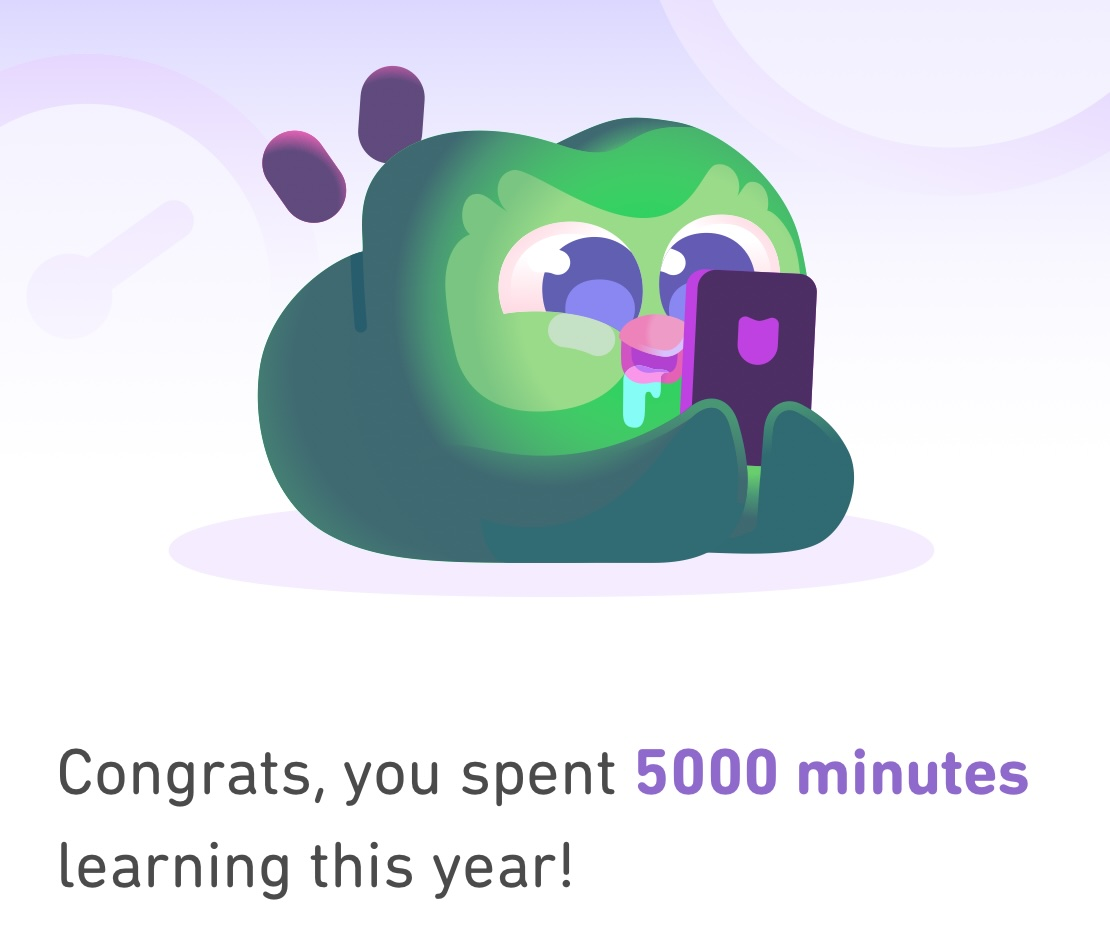
\includegraphics{/images/36-duolingo.jpg}
\end{figure}

I have reached the point of diminishing returns with Duolingo.
I plan to quit it in 2025 after completing a 3000-day streak (I want to quit with style).
If I ever decide to pick up another natural language, I’ll go with \href{https://www.pimsleur.com/}{Pimsleur} instead of Duolingo.
Pimsleur courses require more investment, but they teach you the right things faster.

\section{music}{Music}

As in previous years, I focused on improving my sight-reading skills.
I spent about 150 hours at the piano.
I did not learn any music by heart, but I played a lot of new music without explicitly avoiding memorizing anything.

I only recently realized the difference between reading music and sight-reading it.
It's like your typical Linux versus a hard real-time operating system.
When reading, you can slow down to play things right.
When sight-reading, you need to move on even if you didn't get all the notes right.

In 2025, I'll revise my approach and try a tool that promotes good sight-reading habits, \href{https://pianomarvel.com/}{Piano Marvel}.
I'll also learn a Mozart sonata\sidenote{sn-mozart-sonata}{
  Likely \href{https://www.youtube.com/watch?v=I_AX4R-d29o}{Sonata N16 K. 545} since everyone knows it.
} by heart so that I do not feel embarrassed when people ask me to play something.

\section{sports}{Sports}

2024 was my most active year to date.
I ran more than 3534km, practiced Brazilian Jiu-Jiutsu in more than 150 classes (probably close to 200 hours in total), and lifted weights for over 80 hours.

\begin{figure}[medium-size,center]
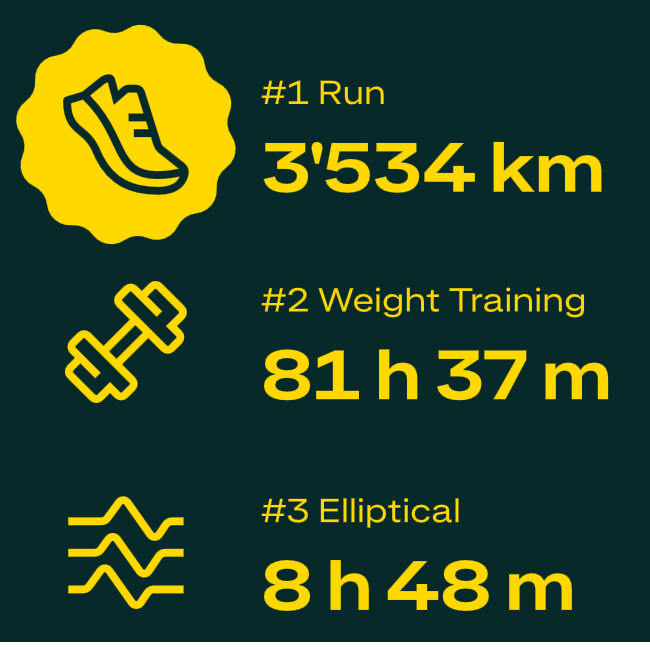
\includegraphics{/images/36-strava.png}
\end{figure}

My most memorable sports event was the Zürich marathon in April, which I finished in 3:32:15, quite a bit faster than I expected.
Most of the distance felt easy and fun, but the last ten kilometers felt pretty miserable, especially since nature decided to shower everyone in rain and snow.

\begin{figure}
\marginnote{mn-marathon-before-after}{
  Me early in the Zürich marathon race and crossing the finish line a few hours later.
}
\center{
    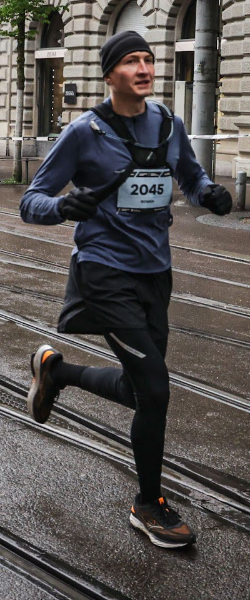
\includegraphics{/images/36-marathon-start.png}
    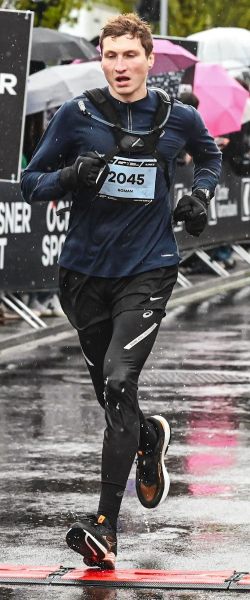
\includegraphics{/images/36-marathon-finish.png}
}
\end{figure}

I also raced two half-marathons (1:40:40 in May and 1:38:38 in September), and improved my time on the \href{https://www.zuerilaufcup.ch/12-laeufe/pfaeffikersee-lauf}{Pfäffikersee-Lauf event} (12.2K) from 59:00 (October 2023) to 54:00 (September 2024).

\href{https://www.goodreads.com/author/show/99585.Matt_Fitzgerald}{Matt Fitzgerald's books} kept me motivated throughout the year, especially \href{https://www.goodreads.com/book/show/49342140-running-the-dream}{Running the Dream}.
I followed one of the half-marathon plans from his \href{https://www.goodreads.com/book/show/58284094-run-like-a-pro-even-if-you-re-slow}{Run Like a Pro (Even If You’re Slow)}, but I overdid it and injured my leg.
Running fast became challenging, so I'll probably wind down my running ambitions in 2025.

BJJ is by far my favorite physical activity.
It's a steady supply of calmness, focus, and hope.
I will keep training in 2025 at least at the same intensity level.
I haven't participated in any competitions yet, and 2025 is a good year to start.

\begin{figure}[medium-size]
\marginnote{mn-bjj}{
  My sensei Joonas (left) and me (right) on the day I got my third stripe.
}
\center{
    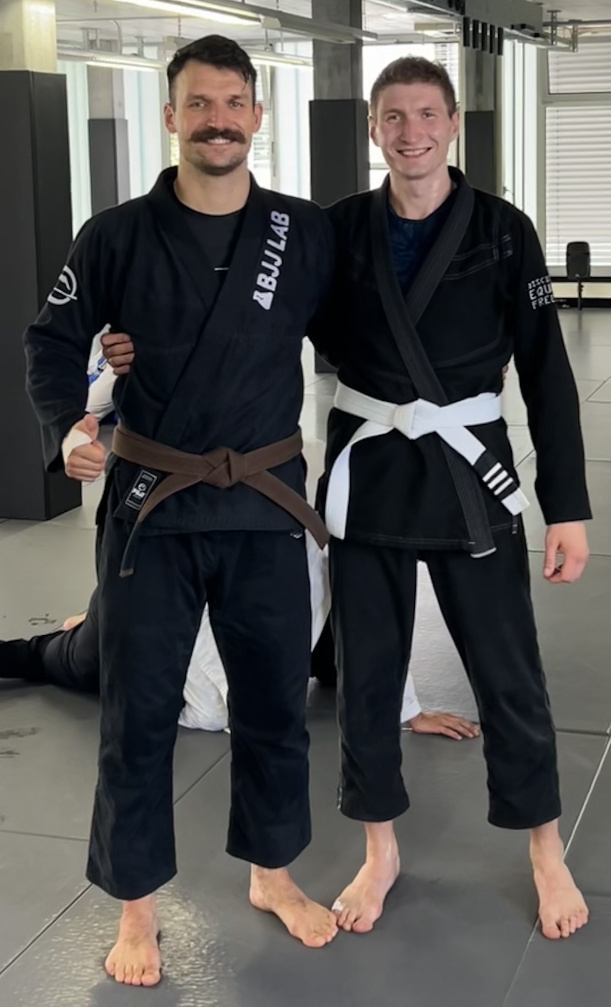
\includegraphics{/images/36-bjj.jpg}
}
\end{figure}

\section{the-most-memorable-day}{The most memorable day}

I conclude this article by describing one day in 2024 that I remember the most.

I had to travel to Paris on a Wednesday in September so the Canadian government could collect my biometrics.
I wanted to resolve the matter in one day, which required about ten hours of commute (about five hours each way).
The day didn't start well: I had to be up with the roosters and could barely walk after a fast run the previous night.
The pain was so intense that I was limping and couldn’t climb the stairs.

The travel time was surprisingly peaceful and productive; the hours flew by.
I reworked one of my early articles, \nameref{05-debug-like-feynman}, and made progress on my tax declaration, which relieved some of my anxiety.

Since the biometrics collection takes at most five minutes,
I didn't have much to do in Paris,
so I roamed the streets,
enjoyed the sunny weather,
sat on a bench in Roger Solengro Park,
and observed kids playing.

On the way back,
I bought presents for my kids, found some tasty butter bread, and listened to a man playing on a slightly out-of-tune piano at La Gare de Lyon before boarding my train to Zürich.

A bit of idleness and quiet solitude transformed a day I dreaded into a highlight of the year.
I didn't get my visa in the end, though.

\end{document}
